\section{Event generation and fit to the $A$-coefficients}
\label{sec:eventsimulation}

\subsection{Simulation setup}



In order to fit the $A$-coefficients, events are generated with the \texttt{ggHH\_SMEFT} implementation of \texttt{Powhex-Box-V2}~\cite{powheg1,powheg2,powheg3,Heinrich:2023rsd}. A grid of 4500 SMEFT points is considered at $\sqrt{s}=13.6$ TeV. The grid is built in two pieces: first, with 2D scans between the Wilson coefficients; second, considering mutual variations of Wilson coefficients in two multi-dimensional Gaussians (one varying $c_\PH,\,c_{\PH \mathrm{kin}},\,c_{u\PH},\,c_{\PH G},\,c_{\PQt G}$, and the other varying all nine parameters) centered on the SM point. The considered ranges are shown on Table \ref{tab:SMEFTcouplings}, where the region covered takes into consideration the global fit constrains described in Refs.~\cite{SMEFiT:2021, Celada:2024mcf}, but with enlarged bounds in order to ensure coverage to regions accessed by searches with less sensitivity. The samples were generated with 50000 events each, using the PDF set \texttt{PDF4LHC15nlo30}\cite{pdf}. The top-quark mass is set to $m_\PQt=173.0$~GeV and is renormalized in the on-shell scheme, while the Higgs boson mass is set to $m_\PH=125.0$~GeV. The renormalization and factorization scales are set to $\mu_R=\mu_F=\mHH/2$. The strong coupling constant $\alpha_s(m_\PZ)=0.118$ is taken from the PDF set and the Wilson coefficients are given at $\Lambda=1$~TeV. The RGE running of the Wilson coefficients is kept switched off in \texttt{Powheg}.




\begin{table}[h!]
\centering
\renewcommand{\arraystretch}{1.2}
\begin{tabular}{c c c c}
\hline
2D scans & 5D Gaussian & 9D Gaussian & Total \\
\hline
$1632$ & $1700$ & $1168$ & $4500$ \\
\end{tabular}
\caption{Grid composition: pairwise two-dimensional scans and multi-dimensional Gaussian centered on the SM. 
}
\label{tab:grids_comp}
\end{table}
\begin{table}[h!]
\centering
\small
\begin{tabular}{|c|c|c|}
\hline
Parameter & Range & SMEFiT name \\
\hline
$c_{\PH}$              & $[\,-50, 50\,]$           & --- \\
$c_{\PH \mathrm{kin}}$ & $[\,-8, 8\,]$               & $c_{\varphi\Box}$, $c_{\varphi D}$ \\
$c_{u\PH}$          & $[\,-10, 7\,]$              & $c_{t\varphi}$ \\
$c_{\PH G}$            & $[\,-0.1, 0.03\,]$     & $c_{\varphi G}$ \\
$c_{\PQt G}$           & $[\,-0.3, 1.0\,]$      & $c_{tG}$ \\
$c_{Q\PQt}^{(1)}$      & $[\,-20, 20\,]$            & $c^{1}_{Qt}$ \\
$c_{Q\PQt}^{(8)}$      & $[\,-20, 20\,]$           & $c^{8}_{Qt}$ \\
$c_{QQ\PQt\PQt}$       & $[\,-20, 20\,]$           & $c^{1}_{QQ}+c^{1}_{tt}$ \\
$c_{QQ}^{(8)}$         & $[\,-20, 20\,]$           & $c^{8}_{QQ}$ \\
%$c_{\PH}$              & $[\,-50, 50\,]$ \\
%$c_{\PH \mathrm{kin}}$ & $[\,-8, 8\,]$ \\
%$c_{u\PH}$          & $[\,-10, 7\,]$ \\
%$c_{\PH G}$            & $[\,-0.1, 0.03\,]$ \\
%$c_{\PQt G}$           & $[\,-0.3, 1.0\,]$ \\
%$c_{Q\PQt}^{(1)}$      & $[\,-20, 20\,]$ \\
%$c_{Q\PQt}^{(8)}$      & $[\,-20, 20\,]$ \\
%$c_{QQ\PQt\PQt}$       & $[\,-20, 20\,]$ \\
%$c_{QQ}^{(8)}$         & $[\,-20, 20\,]$ \\
\hline
\end{tabular}
\caption{Ranges of the Wilson coefficients assumed to derive the $A$-coefficients. The correspondence with SMEFiT \cite{Giani:2023gfq} names is shown in the last column. We use as reference the $95\%$~CI marginalized bounds at $\mathcal{O}(\Lambda^{-4})$ in Refs.~\cite{SMEFiT:2021, Celada:2024mcf}, but with enlarged bounds.}
\label{tab:SMEFTcouplings}
\end{table}
%\begin{table}[h!]
%\centering
%\begin{tabular}{c|c}
%\hline
%Input & Value  \\
%\hline
%Generator          & \texttt{Powheg-Box-V2} at NLO QCD \\
%$m_t$              & $173.0$ GeV \\
%$m_\text{H}$              & $125.0$ GeV \\
%$\mu_{R}=\mu_F$ & $m_{\text{HH}}/2$  \\
%PDF & \texttt{PDF4LHC15\_nlo\_30\_pdfas} \\
%PDF ($100$ TeV)    & \texttt{PDF4LHC21\_40\_pdfas} \\
%$\alpha_s(m_Z)$    & $0.118$ \\
%$\sqrt{s}$         & $13.6$ TeV \\
%$\Lambda$          & $1$ TeV \\
%\hline
%\end{tabular}
%\caption{\texttt{Powheg} input parameters. The top-quark mass is renormalized in the on-shell scheme and the $\alpha_s$ value is taken from the corresponding PDF set. The renormalization and factorization scales are set to $m_{\text{HH}}/2$, and the new physics scale is set to $\Lambda=1$ TeV.}
%\label{tab:POWHEGinput}
%\end{table}

\subsection{Derivation of the coefficients}
\label{sec:a-coeff-derivation}
%\subsubsection{Coefficients at $\sqrt{s}=13.6$ TeV}
The strategy for extracting the $A$-coefficients at $\sqrt{s}=13.6$ TeV follows Ref.~\cite{ELR_R5}, to which we refer for the full discussion of the choice of reweighting variables and of the fitting algorithm. The latter relies in a per bin iteratively reweighted least squares (IRLS) fit, which takes as input all the generated points described in the previous Section. Table \ref{tab:binedge} displays the considered binning, where the 1D-$m_{\HH}$ description in the high-mass region ($m_\HH>1000$ GeV) is needed for ensuring statistical stability. 


\renewcommand{\arraystretch}{1.1}
\begin{table}[t]
\centering
\begin{tabular}{|c|l|}
\hline
Variable & Bin edges \\ \hline
%\multicolumn{2}{|c|}{\textbf{3D}} \\ \hline
$m_{\HH}\:\text{[GeV]}$
& \textcolor{blue}{$250,\:270,\:290,\:310,\:330,\:350,\:370,\:390,\:410,\:430,\:450,\:470,\:490$} \\
& \textcolor{blue}{$510,\:530,\:550,\:570,\:590,\:610,\:630,\:650,\:670,\:690,\:710,\:730,\:750$} \\
& \textcolor{blue}{$800,\:850,\:900,\:950,\:1000$}$,\:1050,\:1100,\:1200,\:1300,\:1400,\:1500,$\\
& $1600,\:1800,\:2000,\:13600$ \\ \hline
$|\cos\theta^*|$
& \textcolor{blue}{$0.0,\:0.25,\:0.5,\:0.75,\:1.0$} \\ \hline
$p^{\HH}_T\:\text{[GeV]}$
& \textcolor{blue}{$0.0,\:20,\:40,\:60,\:80,\:100,\:140,\:200,\:290,\:2500$} \\ \hline
\end{tabular}
\caption{Bin edges considered. The blue color indicates where binning is 3D. The high-mass region ($m_{\text{HH}}>1000$ GeV) it is always one-dimensional due to the lack of statistics.}
\label{tab:binedge}
\end{table}
\renewcommand{\arraystretch}{1.0}
\begin{figure}[h!]
  \centering
  % First group: 2 x 2
  \begin{minipage}[b]{0.495\linewidth}
    \centering
    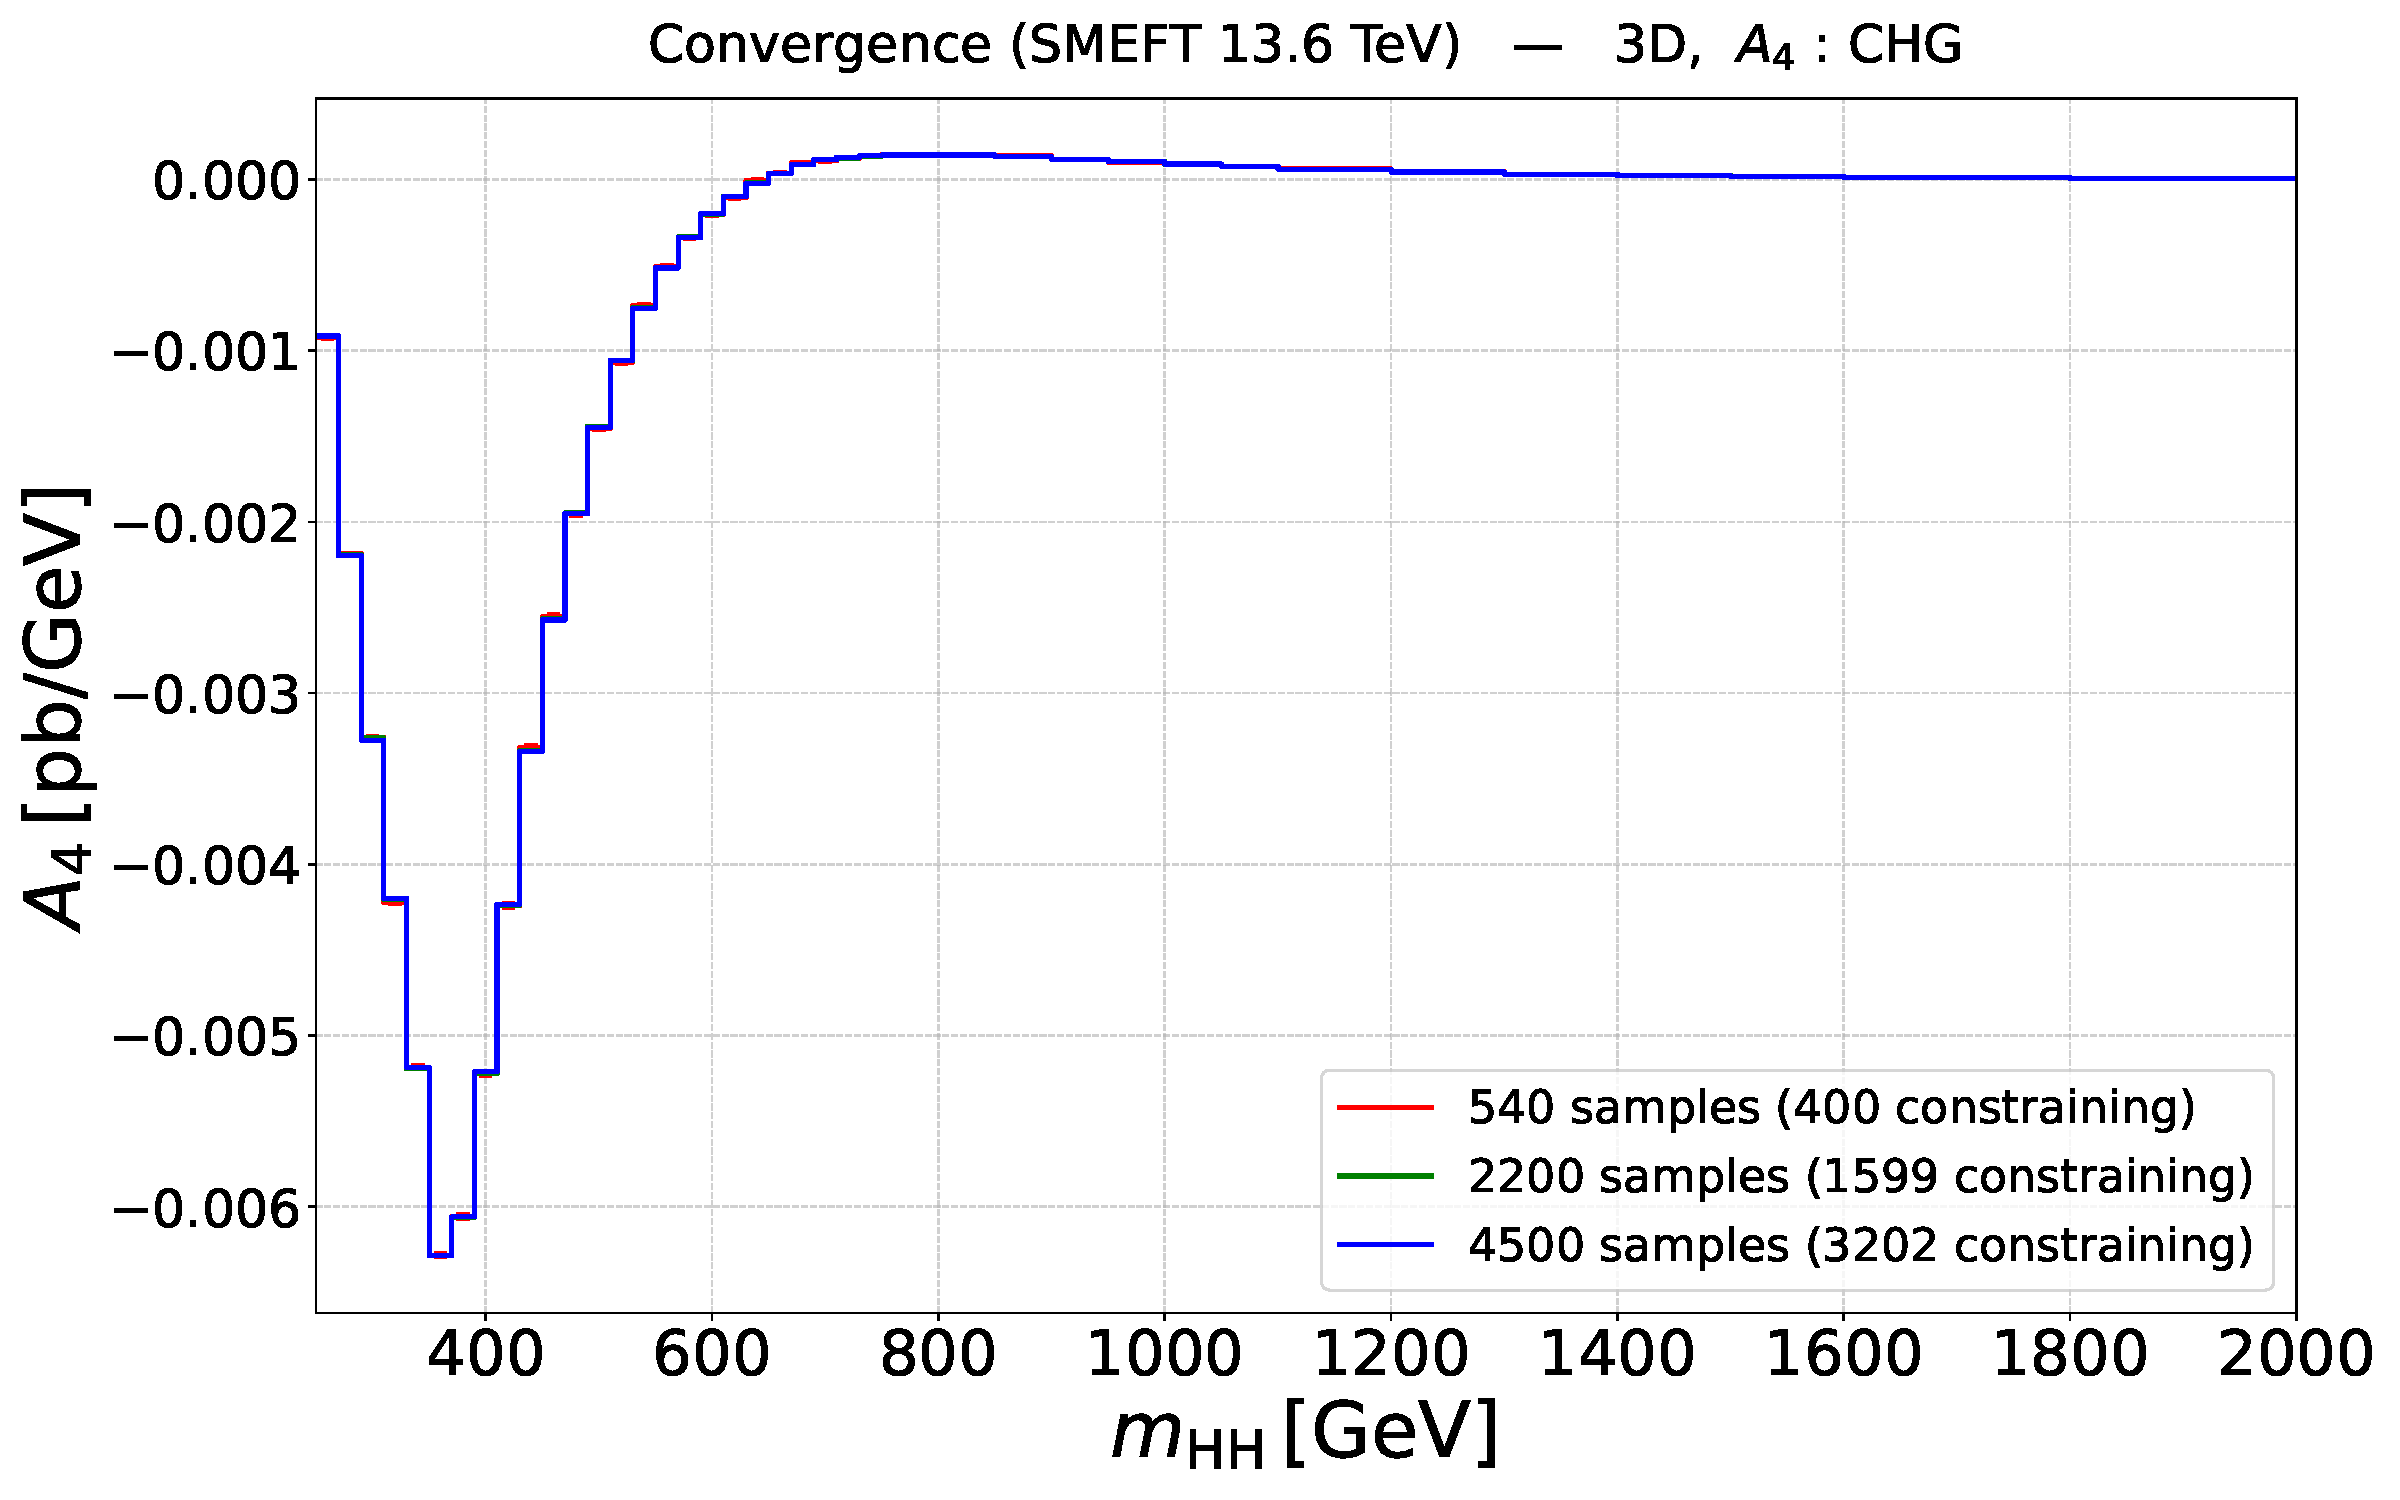
\includegraphics[width=\linewidth]{plots/plot_param4_250_2000_3d_convergence_9D.pdf}
  \end{minipage}
  \hfill
  \begin{minipage}[b]{0.495\linewidth}
    \centering
    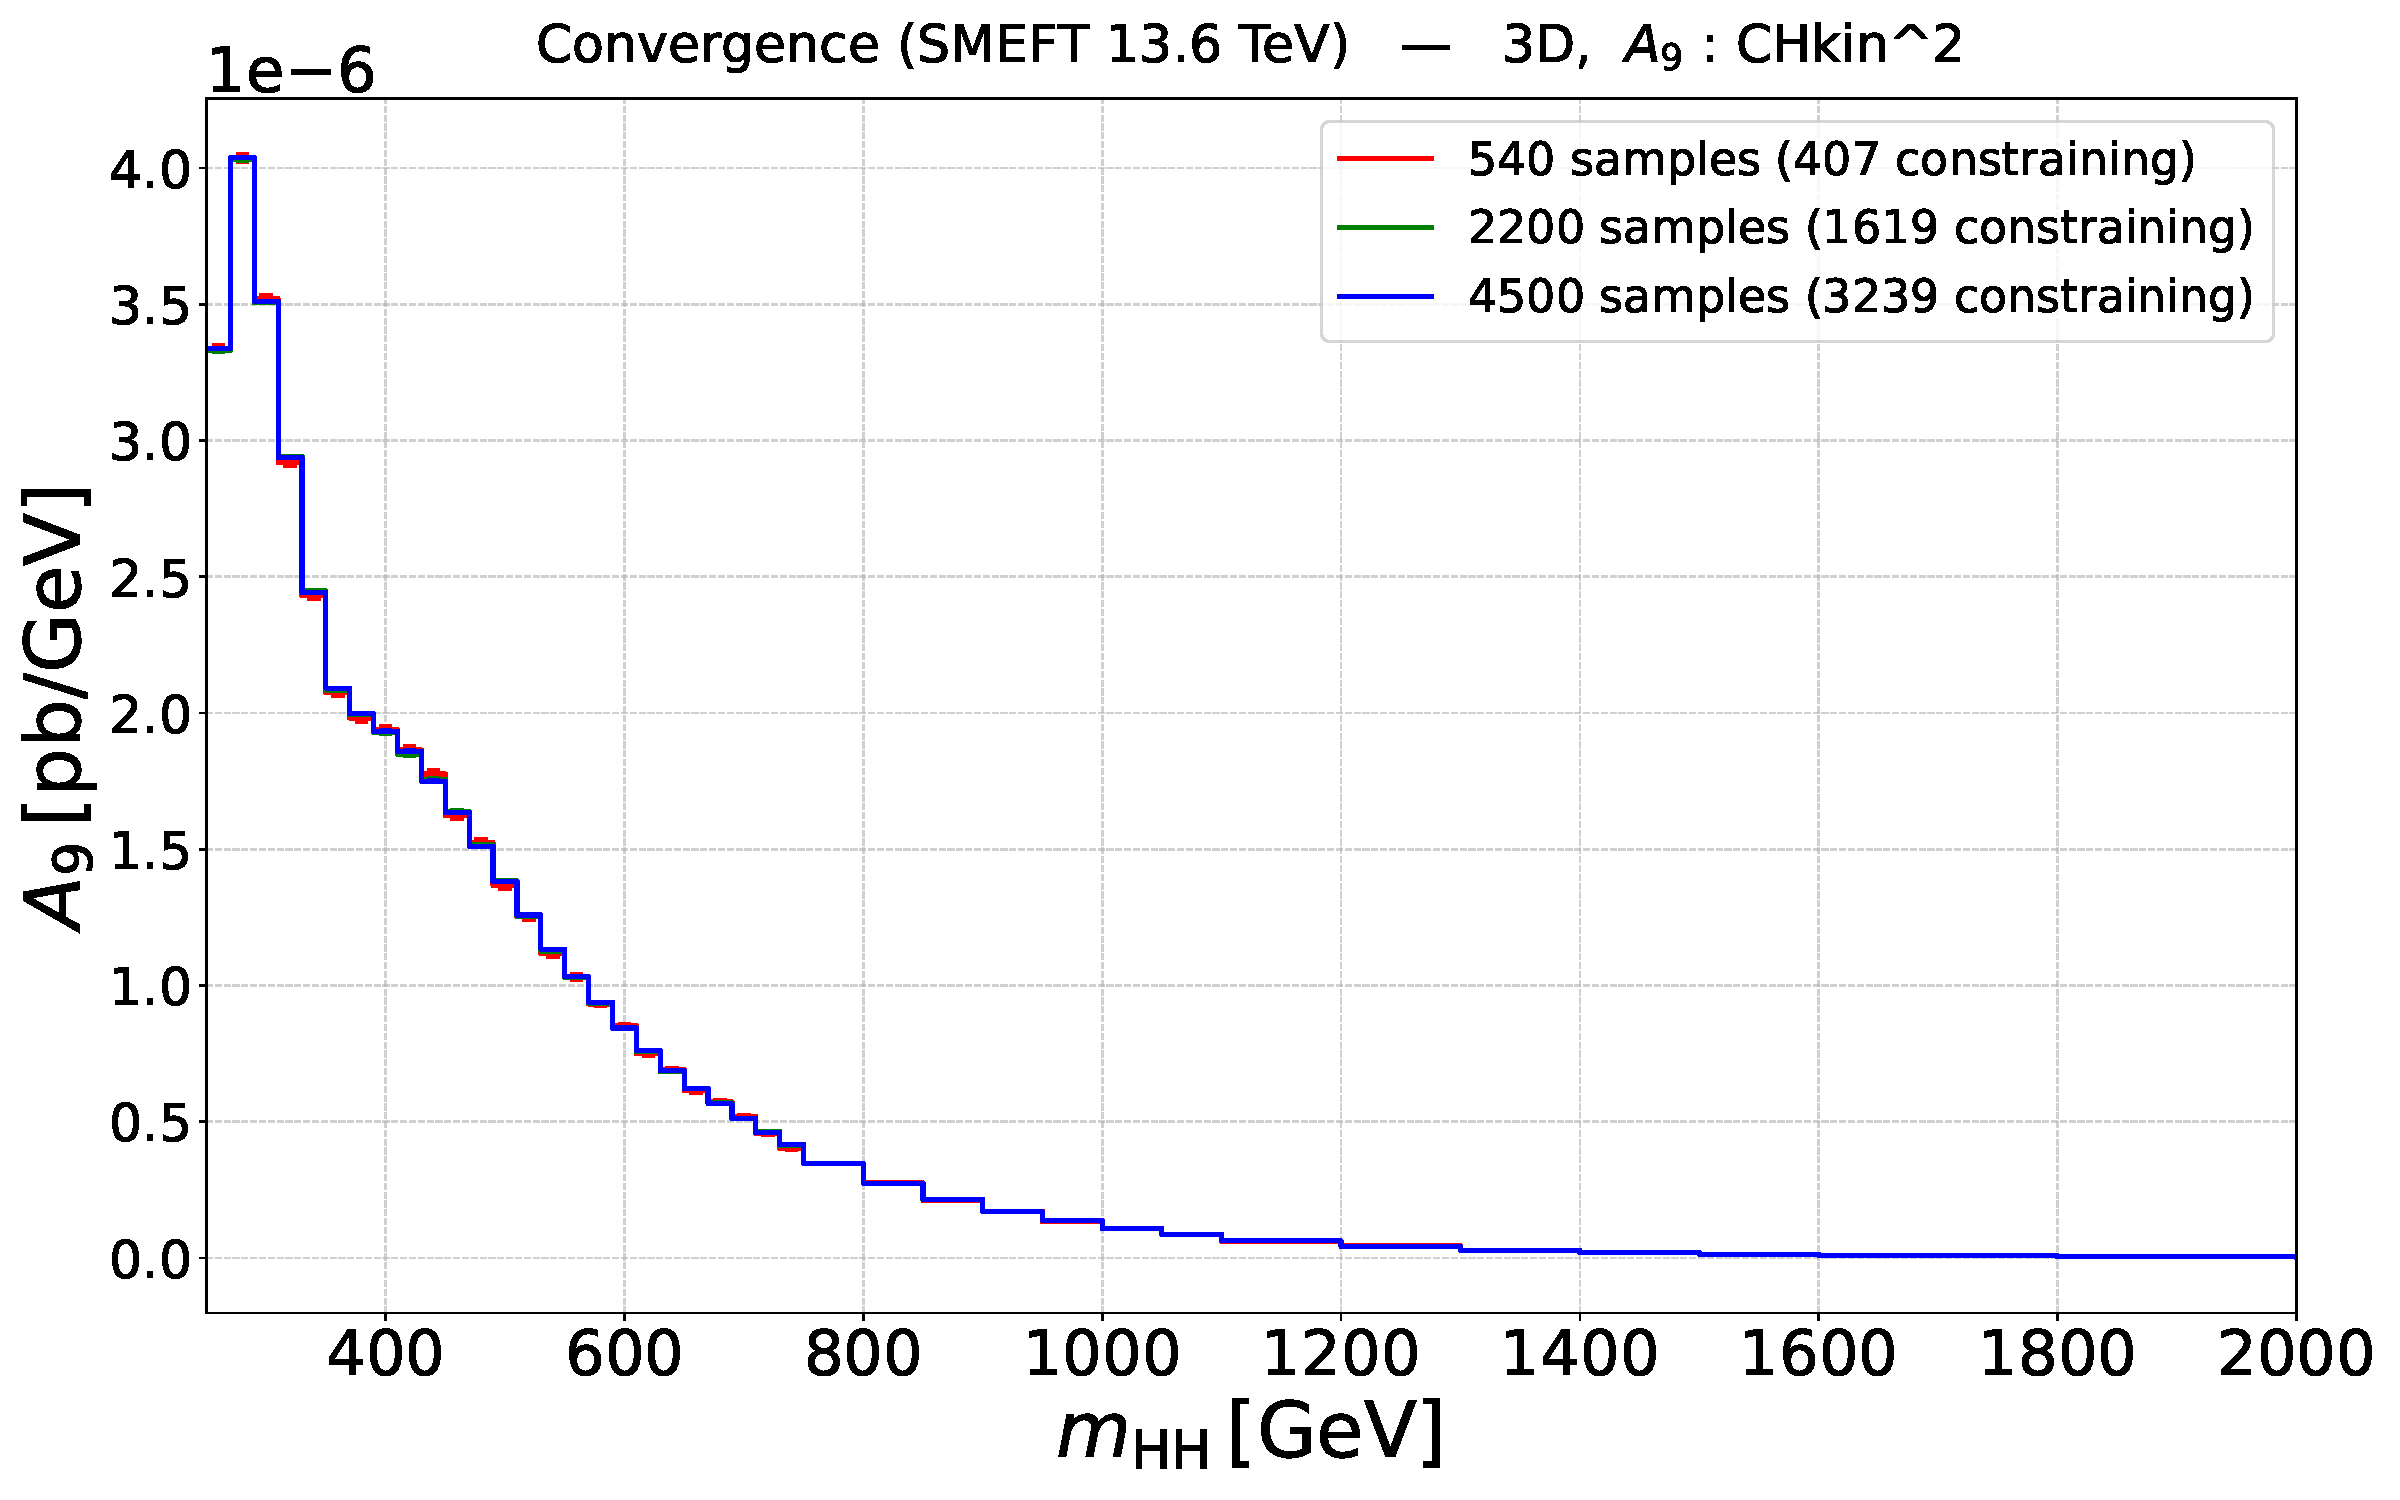
\includegraphics[width=\linewidth]{plots/plot_param9_250_2000_3d_convergence_9D.pdf}
  \end{minipage}
  \vspace{0.5em}
  \begin{minipage}[b]{0.495\linewidth}
    \centering
    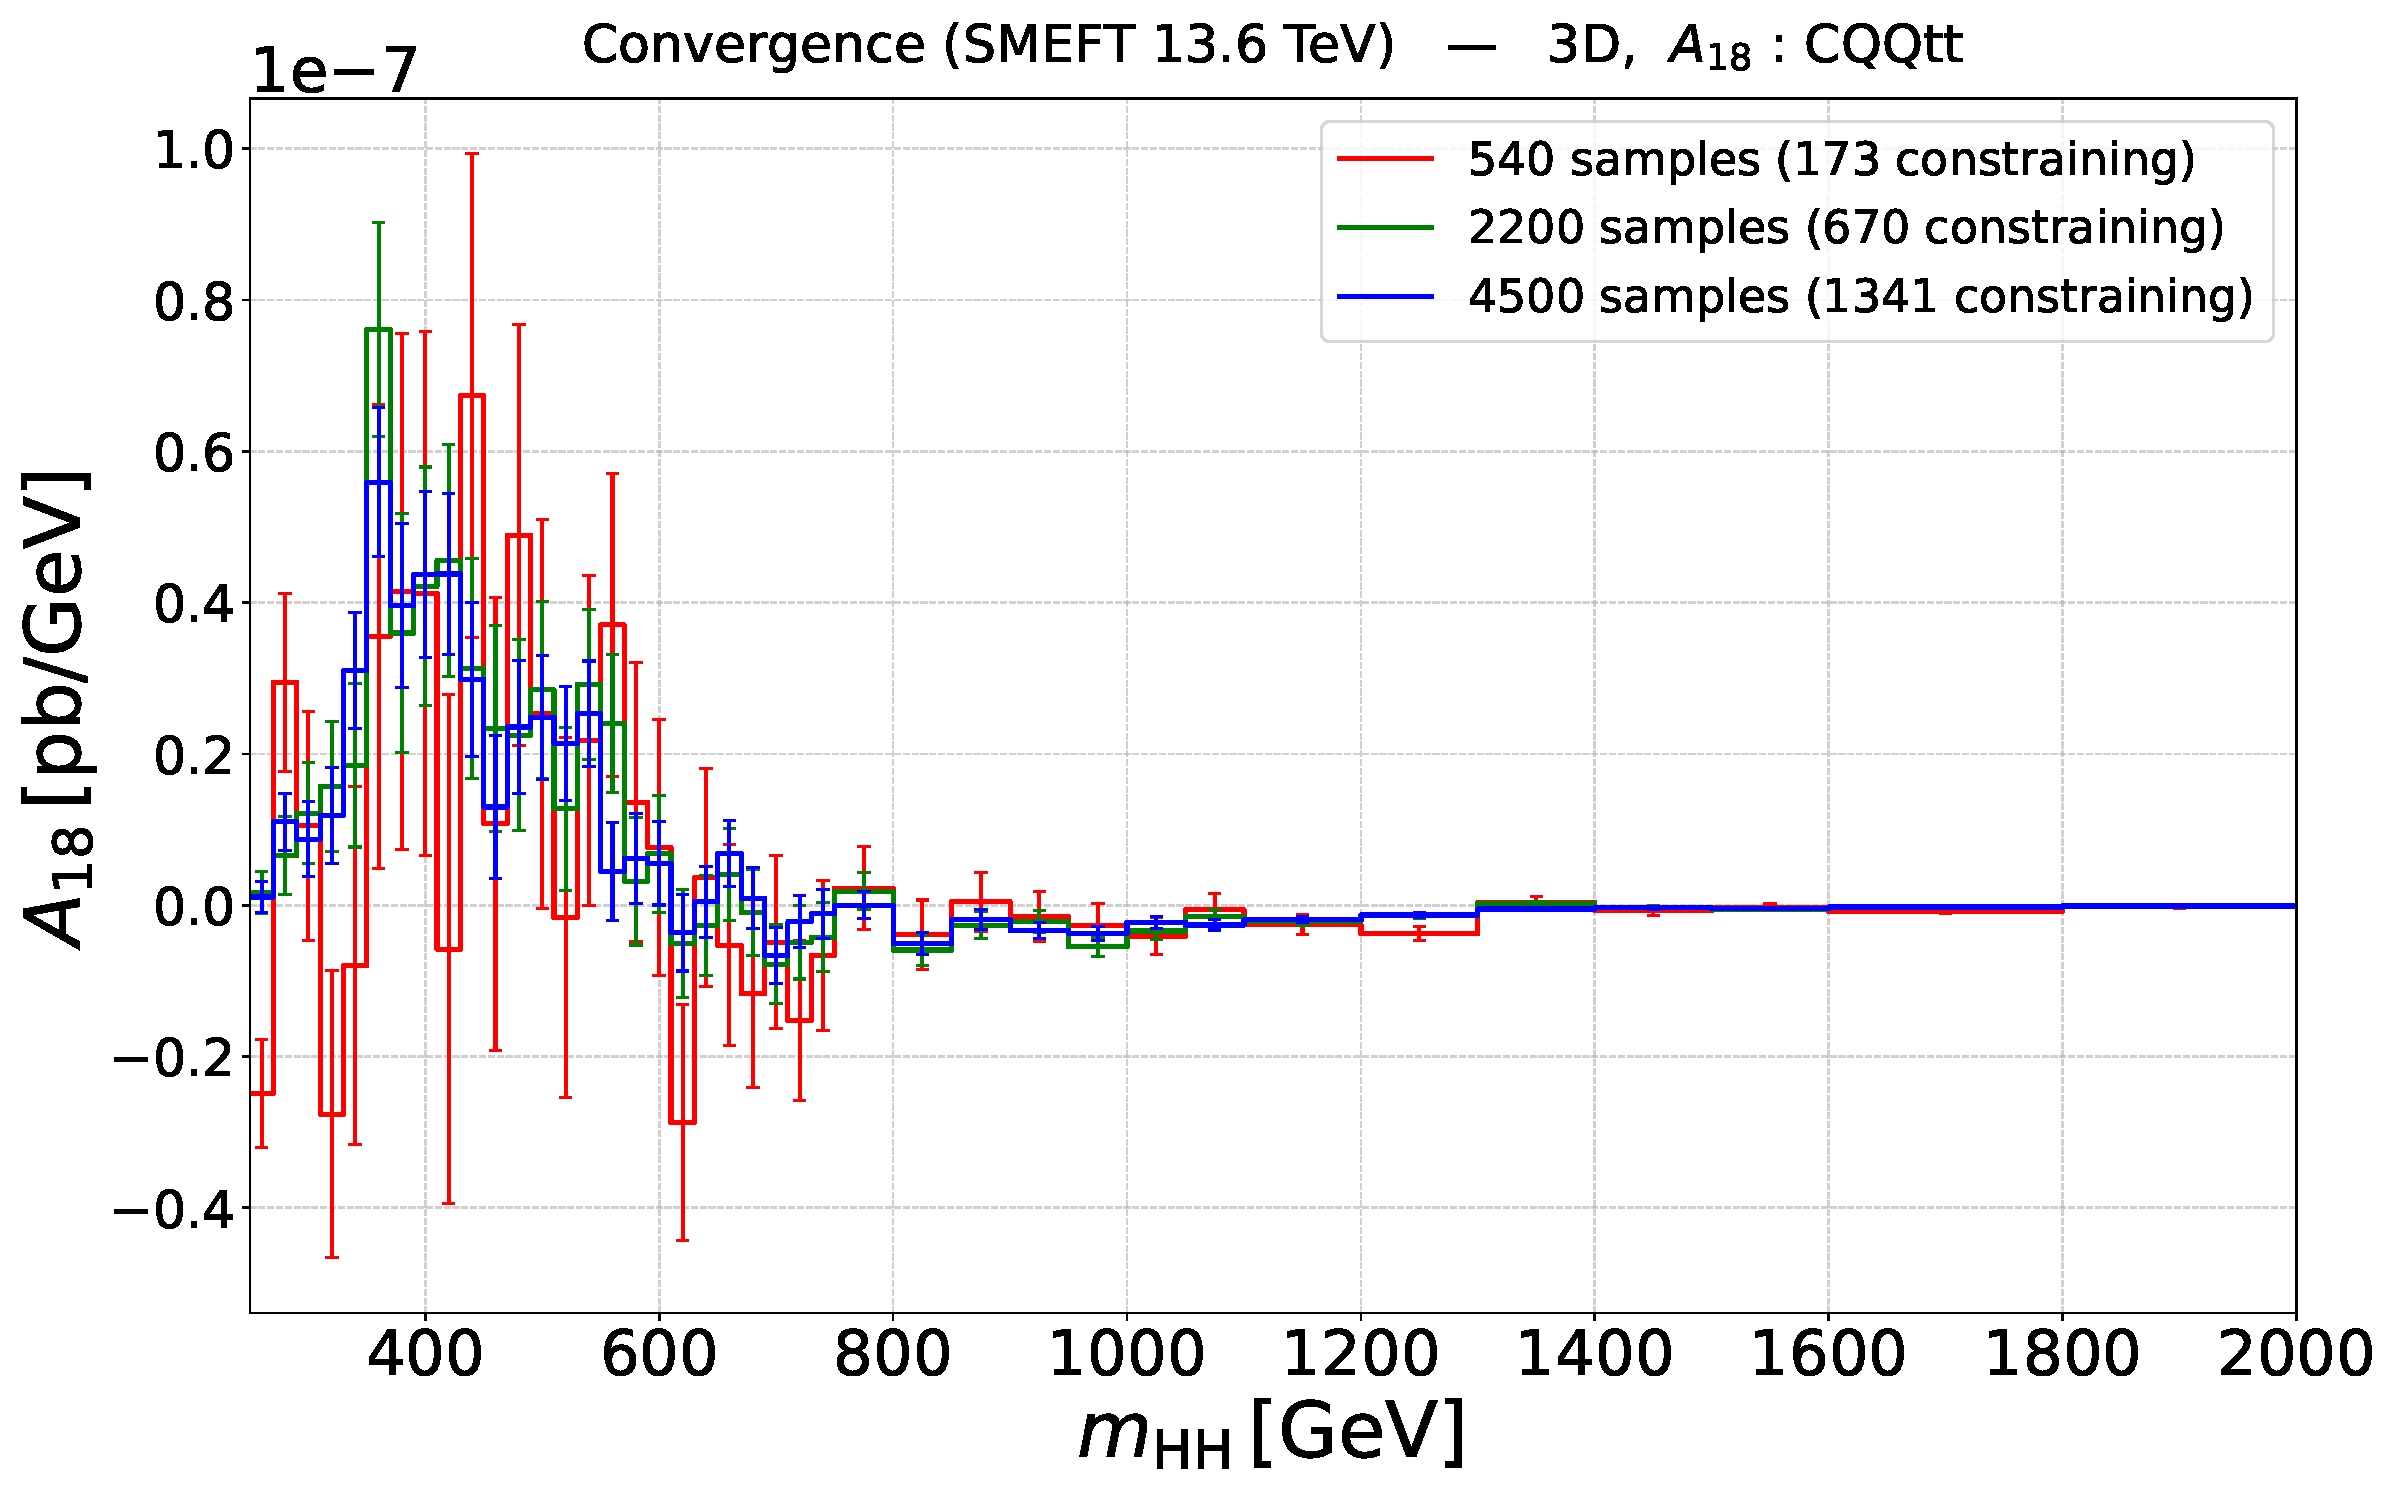
\includegraphics[width=\linewidth]{plots/plot_param18_250_2000_3d_convergence_9D.pdf}
  \end{minipage}
  \hfill
  \begin{minipage}[b]{0.495\linewidth}
    \centering
    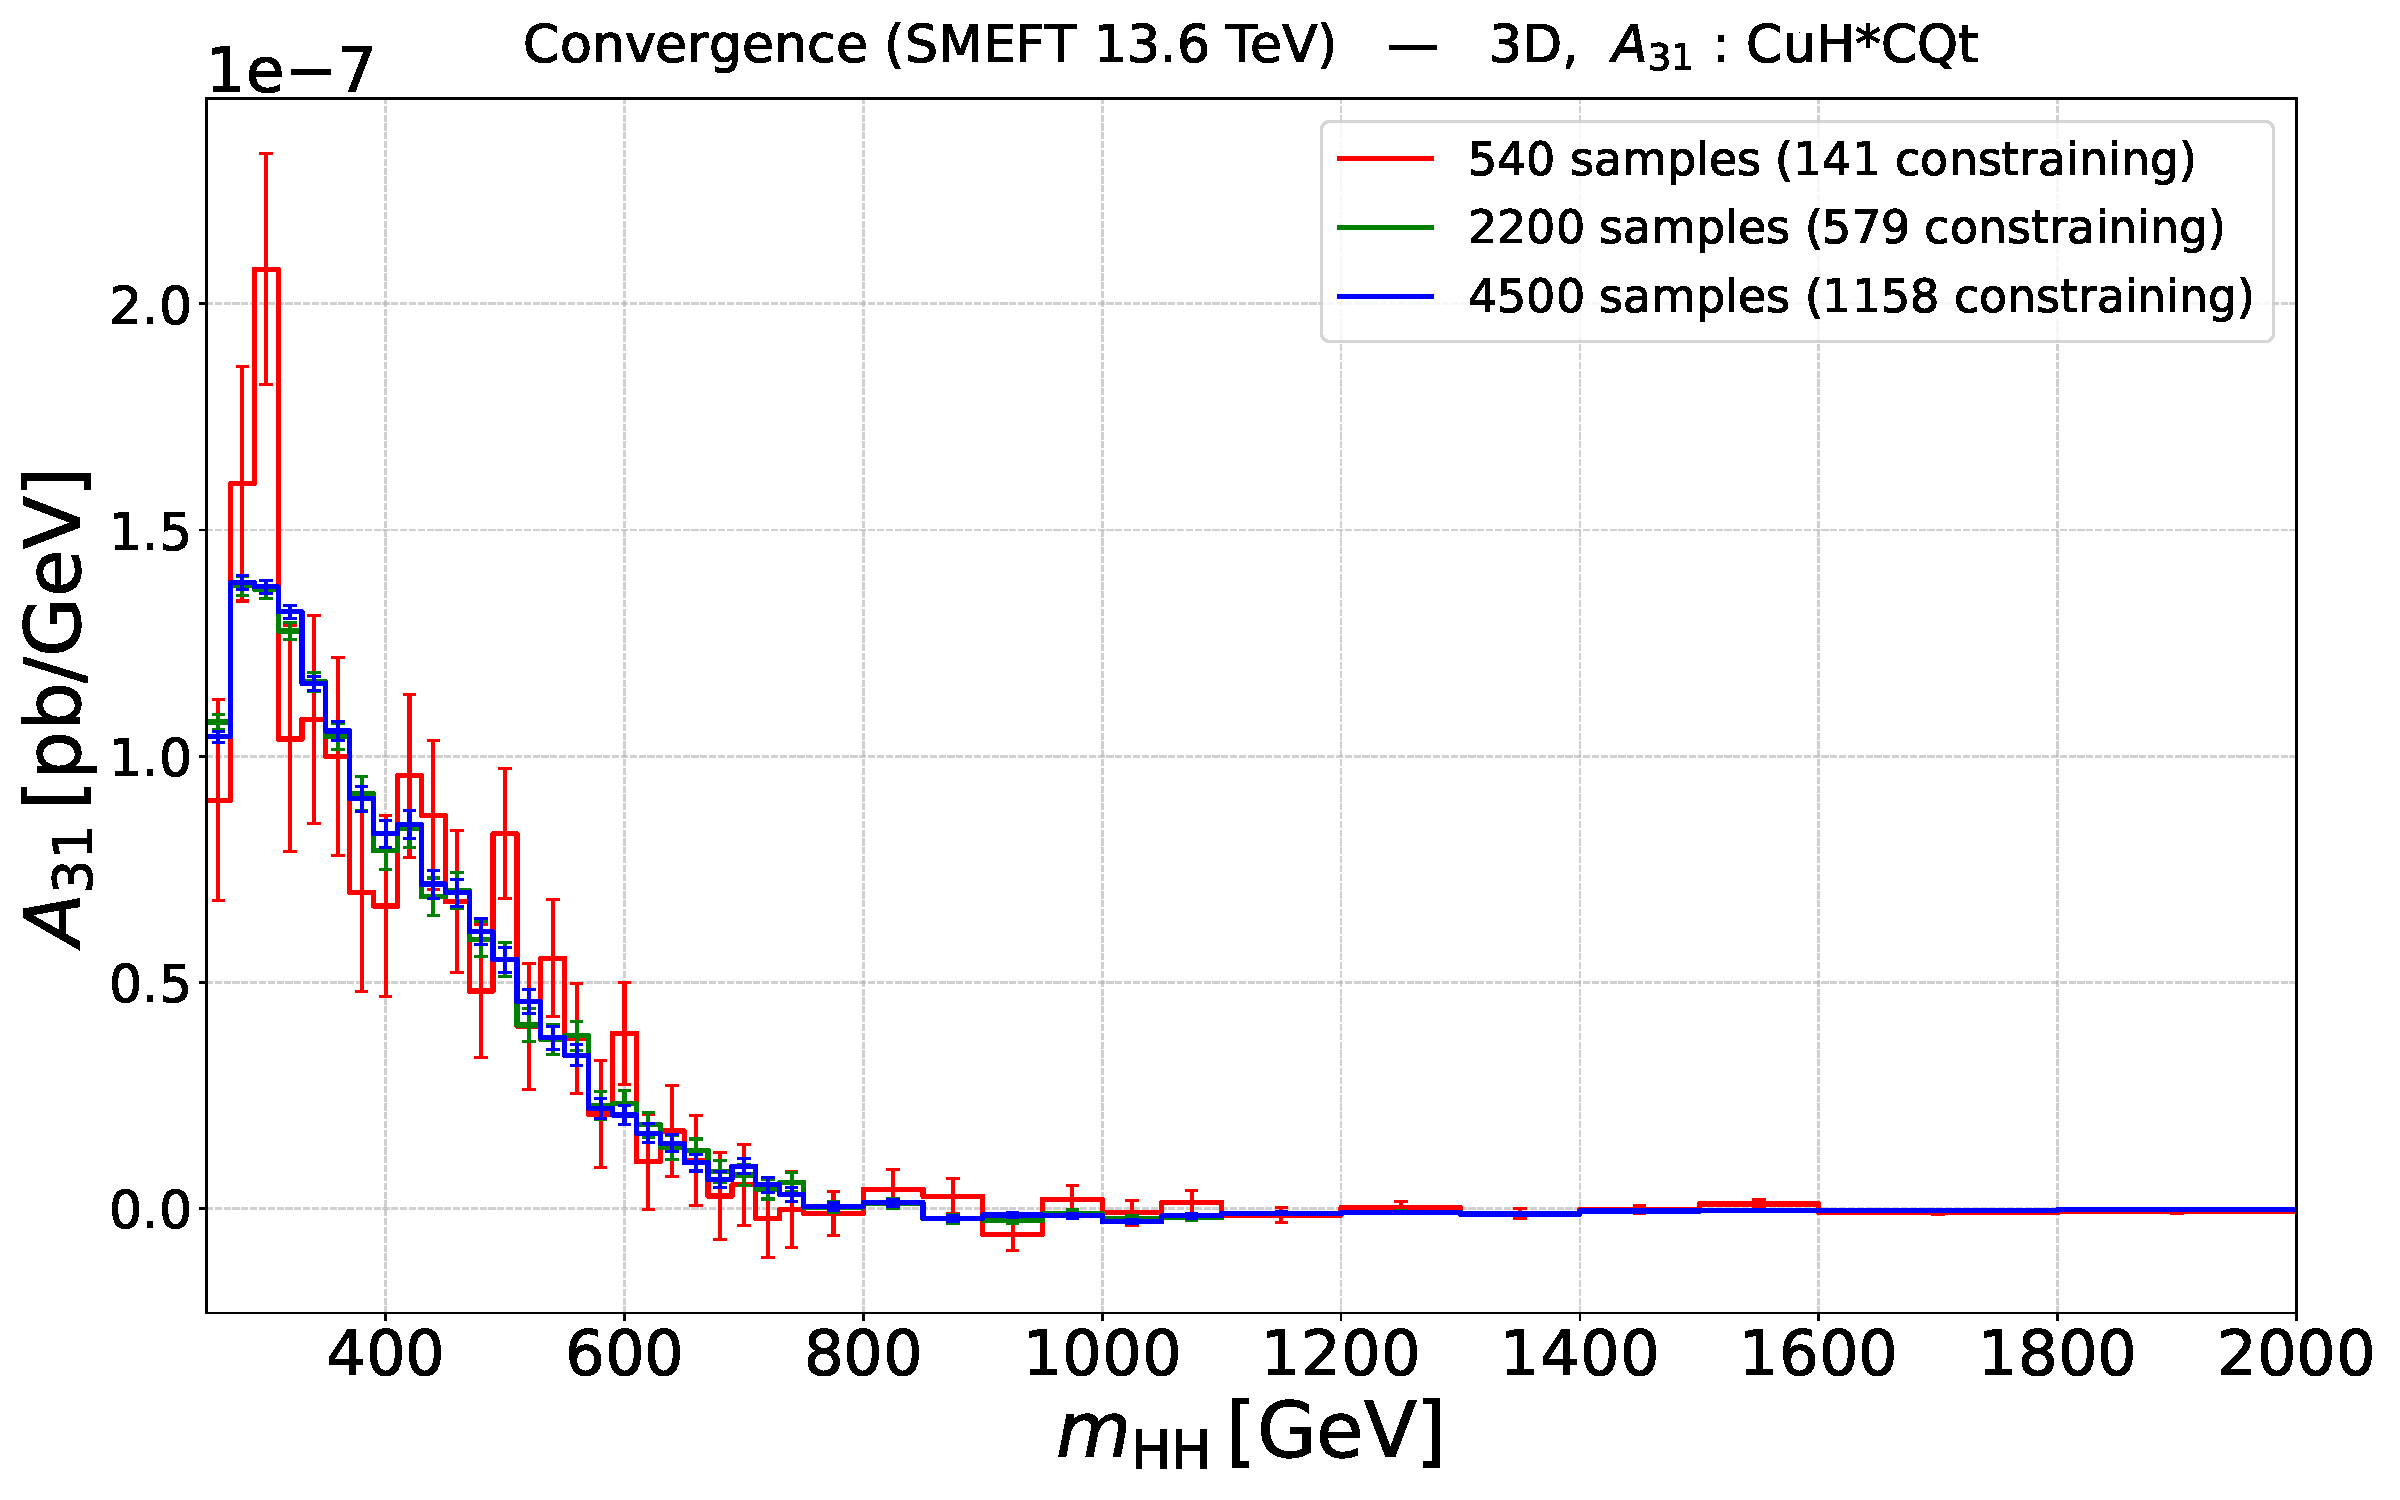
\includegraphics[width=\linewidth]{plots/plot_param31_250_2000_3d_convergence_9D.pdf}
  \end{minipage}
  \caption{Convergence of the 3D $A$-coefficients projected into $m_{\text{HH}}$. The upper panel shows coefficients arising from leading-operator terms, while the lower panel shows coefficients arising from subleading and leading$\times$subleading terms.}
  \label{fig:convergence}
\end{figure}

The convergence of some of the coefficients is exhibited in Fig.~\ref{fig:convergence}. All coefficients stemming from leading-only operator insertions show quick convergence, as represented by the upper panel. On the other hand, all coefficients involving subleading components require more samples to stabilize, regardless coming from linear (bottom-left) or quadratic (bottom-right) contributions.

The final set of coefficients consistent with the updated PDF set (\texttt{PDF4LHC21\_40} \cite{PDF4LHC21}) and at all COM energies $\sqrt{s}=13$,  $13.6$, $14$ TeV, are obtained with the transport technique discussed in Ref.~\cite{ELR_R5}, and the validation of this procedure in SMEFT is shown in Appendix ~\ref{sec:validation_transport}. All set of coefficients and the corresponding covariance matrices are available as supplementary files in the arXiv submission.


%\subsubsection{Coefficients at $\sqrt{s}=13$ and $14$ TeV}
%The coefficients at $\sqrt{s}=13$ and $14$ TeV can be derived from the $13.6$ TeV ones by applying transfer factors that account for the effects of the PDFs at different COM energies. For a given generated event, the subprocess final state kinematics (e.g. $\{m_{\HH},|\cos\theta^*|,p^\HH_T|$) are fixed. Therefore, with $\hat{s}=x_1x_2s$ and $y=\frac{1}{2}\ln{(x_1/x_2)}$ held constant, a change in the COM energy implies in scaling the momentum fractions with $x^\prime_i=x_i\sqrt{s/s^\prime}$ and can be factorized as
%\begin{equation}\label{eq:transport}
%    \frac{d\sigma(\sqrt{s}^\prime)/d\hat{s}dy}{d\sigma(\sqrt{s})/d\hat{s}dy}=\frac{s}{s^\prime}\frac{f(x^\prime_1,\mu_F)f(x^\prime_2,\mu_F)}{f(x_1,\mu_F)f(x_2,\mu_F)},
%\end{equation}
%which depends only on initial state quantities. From the parameterization shown in Eq.~\eqref{eq:smeftpara_reorg}, this is to say that the $A$-coefficients can be scaled with per bin transfer factors that multiplies all the 40 terms:
%\begin{equation}
%    A^i_j(\sqrt{s}=13,14\text{ TeV})=T_jA^i_j(\sqrt{s}=13.6 \text{ TeV}).
%\end{equation}
%These factors can be extracted by accessing the initial state partons in the generated events at $\sqrt{s}=13.6$ TeV, to which one can use the $x\to x^\prime$ transport to get both the numerator and denominator in Eq.~\eqref{eq:transport}. Once this is computed for all events, the per bin $T$-factors are then extracted and used to rescale the $A$-coefficients to both $13$ and $14$ TeV. For a given bin $j$, the covariance matrices are accordingly scaled as
%\begin{equation}
%C_{kl}(\sqrt{s}',j) = T_j^2 \left[ C_{kl}(\sqrt{s},j)
%                      + r_j^2\, A_k^j A_l^j \right],
%\label{eq:energy_cov}
%\end{equation}
%since $cov(TA_k,TA_l)=T^2cov(A_k,A_j)$. The second term is due to the statistical uncertainty $r_j$ in the extraction of the $T_j$-factor.


%The new coefficients are validated with additional samples generated at the corresponding COM energies and found to provide the same level of accuracy as the fitted coefficients in $13.6$ TeV, but without requiring the generation of thousand of new samples for new dedicated fits. Additional details and validation of this procedure is provided in Appendix~\ref{sec:validation_transport}.    

%The 3D coefficients at all three energies, together with their covariance matrices, are available as ancillary files in the arXiv submission.


%\subsection{Linear and quadratic truncations}

%The coefficients are also validated against benchmark points generated separately in the linear and in the quadratic truncation, which is the subject of Sec.~\ref{sec:truncation}.

%\newpage
%\subsection{Renormalization-group running of the Wilson coefficients}
%The RGE running of the Wilson coefficients is kept \emph{switched off} in
%\texttt{Powheg}, and the coefficients are taken at the fixed scale $\Lambda=1$~TeV
%throughout. This is a deliberate choice, not a simplification of convenience.
%With running enabled the coefficients entering the matrix element become
%$c_i(\mu_{\text{EFT}})$ evaluated at the dynamical scale $\mu_{\text{EFT}}=\mHH/2$,
%so every generated event carries a different effective set of couplings. The
%$A$-coefficients of Eq.~\eqref{eq:smeftpara_reorg} would then no longer be pure
%numbers attached to the process: they would absorb the running, become specific to
%one choice of $\Lambda$ and one running implementation, and lose the property that
%makes the parameterization useful in the first place --- that a user can evaluate
%the same polynomial at any coefficient point without regenerating anything. Since
%$\mu_{\text{EFT}}$ is tied to \mHH, the effect does not even factorize between the
%inclusive and the differential parameterizations.

%The effects themselves are not negligible at the precision these templates aim
%for, and are becoming a standard part of SMEFT
%interpretations~\cite{Maltoni:2024dpn,terHoeve:2025rge}. They are, however,
%recoverable after the fact, and this is worth stating explicitly because it is the
%reason the choice above costs nothing. At leading logarithmic accuracy the
%solution of the dimension-6 RGEs is \emph{linear} in the Wilson coefficients,
%\begin{equation}
%c_i(\mu) = U_{ij}(\mu,\Lambda)\,c_j(\Lambda),
%\qquad
%U_{ij}(\mu,\Lambda) = \delta_{ij} + \frac{\gamma_{ij}}{16\pi^2}\ln\frac{\mu}{\Lambda}
%+ \mathcal{O}(\ln^2) ,
%\label{eq:rge_linear}
%\end{equation}
%with $\gamma_{ij}$ the anomalous-dimension matrix. A linear map composed with a
%quadratic polynomial is again a quadratic polynomial, so the templates extracted
%with running off can be used to obtain the running result simply by evaluating
%them at the transformed coefficient vector $U(\mu,\Lambda)\,c(\Lambda)$, with
%$U$ obtained from any of the standard solvers. Two conditions apply. First, the
%transformation must be done \emph{differentially}, bin by bin in \mHH, using
%$\mu=\mHH/2$ in each bin, since that is the scale the running would have used;
%applying a single inclusive $U$ is not equivalent. Second, Eq.~\eqref{eq:rge_linear}
%propagates the running of the nine coefficients among themselves, but the RGEs also
%generate operators outside this set, and those contributions are not captured by a
%polynomial spanning only the nine. Their size has to be checked rather than
%assumed --- for \ggHH the relevant mixing is dominated by the top-quark Yukawa and
%gauge contributions, which stay within the set, but that statement should be
%verified before the correction is quoted as complete.

%\textcolor{red}{TO DO: quantify this. Regenerating a small subset of points with
%running enabled and comparing against the templates evaluated at
%$U(\mHH/2,\Lambda)\,c(\Lambda)$ would both validate the recovery procedure and
%bound the out-of-basis contribution. This is cheap and would turn the argument
%above into a measurement.}

